\chapter{Pool D (Mobile) --- Feature 9: Discount Coupon}

\section{Phạm vi và test oracle}

Pool D kiểm thử Discount Coupon tại Mobile checkout theo FR-08, FR-09 và các
GUI rule liên quan. Oracle bao gồm năm điều kiện C1--C5, công thức percent/fixed,
trusted total, authentication/identity, usage limit và số tiền cuối cùng. Source
Mobile và Backend chỉ được dùng để tìm đường thực thi/root cause, không thay thế
requirement.

Hai mươi rule \texttt{D-R01}--\texttt{D-R20} được mô hình hóa thành partition,
state transition và sáu nhóm boundary. Các nội dung chưa có oracle như trim/case,
loading/double tap, reset-on-edit, rounding/cap/floor, resilience và native
semantic được giữ thành gap, không bị viết lại theo implementation.

\section{Môi trường và giới hạn nền tảng}

Lượt thực thi chính thức chạy từ 19:32:01 đến 19:32:59 ngày 15/10/2026.
Expo Web chạy tại \url{http://127.0.0.1:8081}; Backend chạy tại
\url{http://127.0.0.1:3000}. Trình duyệt là Chromium hệ thống với viewport
Mobile \(440 \times 956\). Automation dùng Playwright với SQLite fixture cô lập,
reset trước mỗi case. Hash trước/sau xác nhận source SHOP và database gốc không
bị runner sửa.

Lượt chạy chuẩn không dùng emulator, Expo Go hoặc thiết bị thật. Ngày 16/10/2026,
9 screenshot bổ sung được chụp trên một thiết bị iOS thật qua Expo Go/Expo SDK 57
và endpoint API qua LAN. Model thiết bị và phiên bản iOS chưa được ghi nhận. Do
dependency/cấu hình khác baseline, bộ ảnh chỉ corroborate kết quả, không thay thế
lượt chạy chuẩn hoặc làm thay đổi verdict.

\section{Smoke test ban đầu}

Ảnh ngày 09/10/2026 lúc 10:48 AM cho thấy checkout và coupon accessible trên
Expo Web với Chrome device emulation. Đây là smoke evidence, không phải verdict
test case.

\begin{figure}[H]
  \centering
  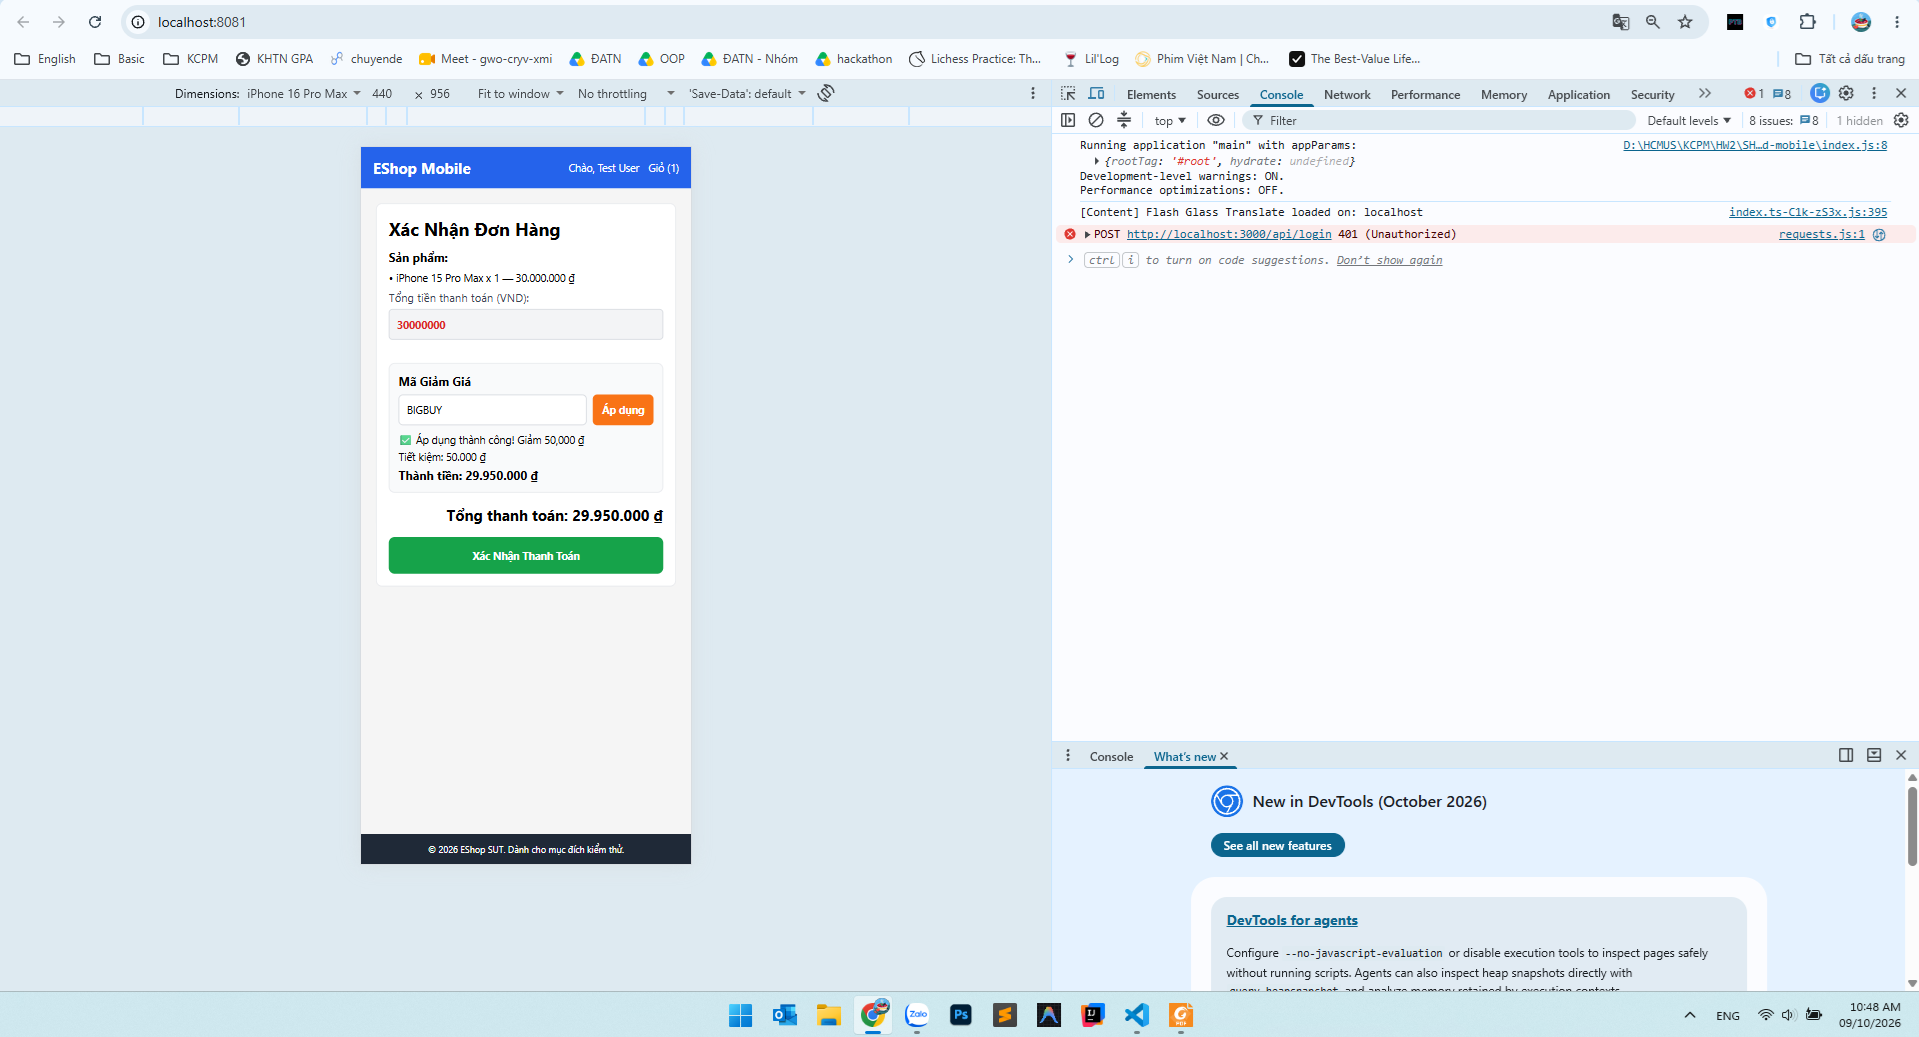
\includegraphics[width=0.92\textwidth,height=0.62\textheight,keepaspectratio]{../../evidence/D/smoke/D-M09-SMOKE-001-mobile-coupon.png}
  \caption{D-M09 --- Smoke evidence trên Expo Web với viewport Mobile.}
  \label{fig:d-m09-mobile-coupon-smoke}
\end{figure}

\section{Domain Testing và BVA}

Equivalence Partitioning bao phủ code/state coupon, authentication, usage,
transport, arithmetic output, UI conformance và environment. BVA dùng các điểm
dưới--bằng--trên cho order minimum, expiry và usage limit; discount value dùng
phía âm, zero và giá trị dương nhỏ nhất. Trust-boundary test tách total và
\texttt{user\_id} do client gửi khỏi authoritative server/JWT value.

Design coverage đạt \texttt{20/20} rule và liên kết đủ \texttt{6/6} boundary.
Đây là design coverage, không phải execution/native coverage 100\%.

\section{Automation và kết quả thực thi}

Runner tại \path{automation/D-M09} chạy tuần tự 50 test case, tự khởi động
Backend/Expo Web, lưu screenshot và Playwright trace cho từng case, đồng thời
xuất \path{evidence/D/execution/results.json} và service log.

\begin{table}[H]
  \centering
  \small
  \begin{tabular}{lrrrrrr}
    \toprule
    Designed & Executed & Pass & Fail & Blocked & Not Run & Execution coverage \\
    \midrule
    50 & 30 & 19 & 11 & 20 & 0 & 60.00\% \\
    \bottomrule
  \end{tabular}
  \caption{Kết quả thực thi D-M09 trên Expo Web.}
  \label{tab:d-m09-results}
\end{table}

\texttt{Executed = PASS + FAIL}. Tỷ lệ PASS trong 30 case có verdict là
\(19/30=63.33\%\), nhưng không phải tiêu chí chấp nhận feature khi còn FAIL và
BLOCKED.

Evidence native bổ sung gồm 5 ảnh bám đúng procedure, 2 ảnh dùng test data khác
thiết kế và 2 ảnh observation-only. Các ảnh chứng minh app có thể gọi Backend
trên iOS thật và cho thấy một số trạng thái UI/keyboard, nhưng không phải native
automation trace.

\begin{figure}[H]
  \centering
  
\includegraphics[width=0.42\textwidth,height=0.60\textheight,keepaspectratio]{../../evidence/D/native-ios/screenshots/D-TC-001-ios-physical.jpg}\hfill
  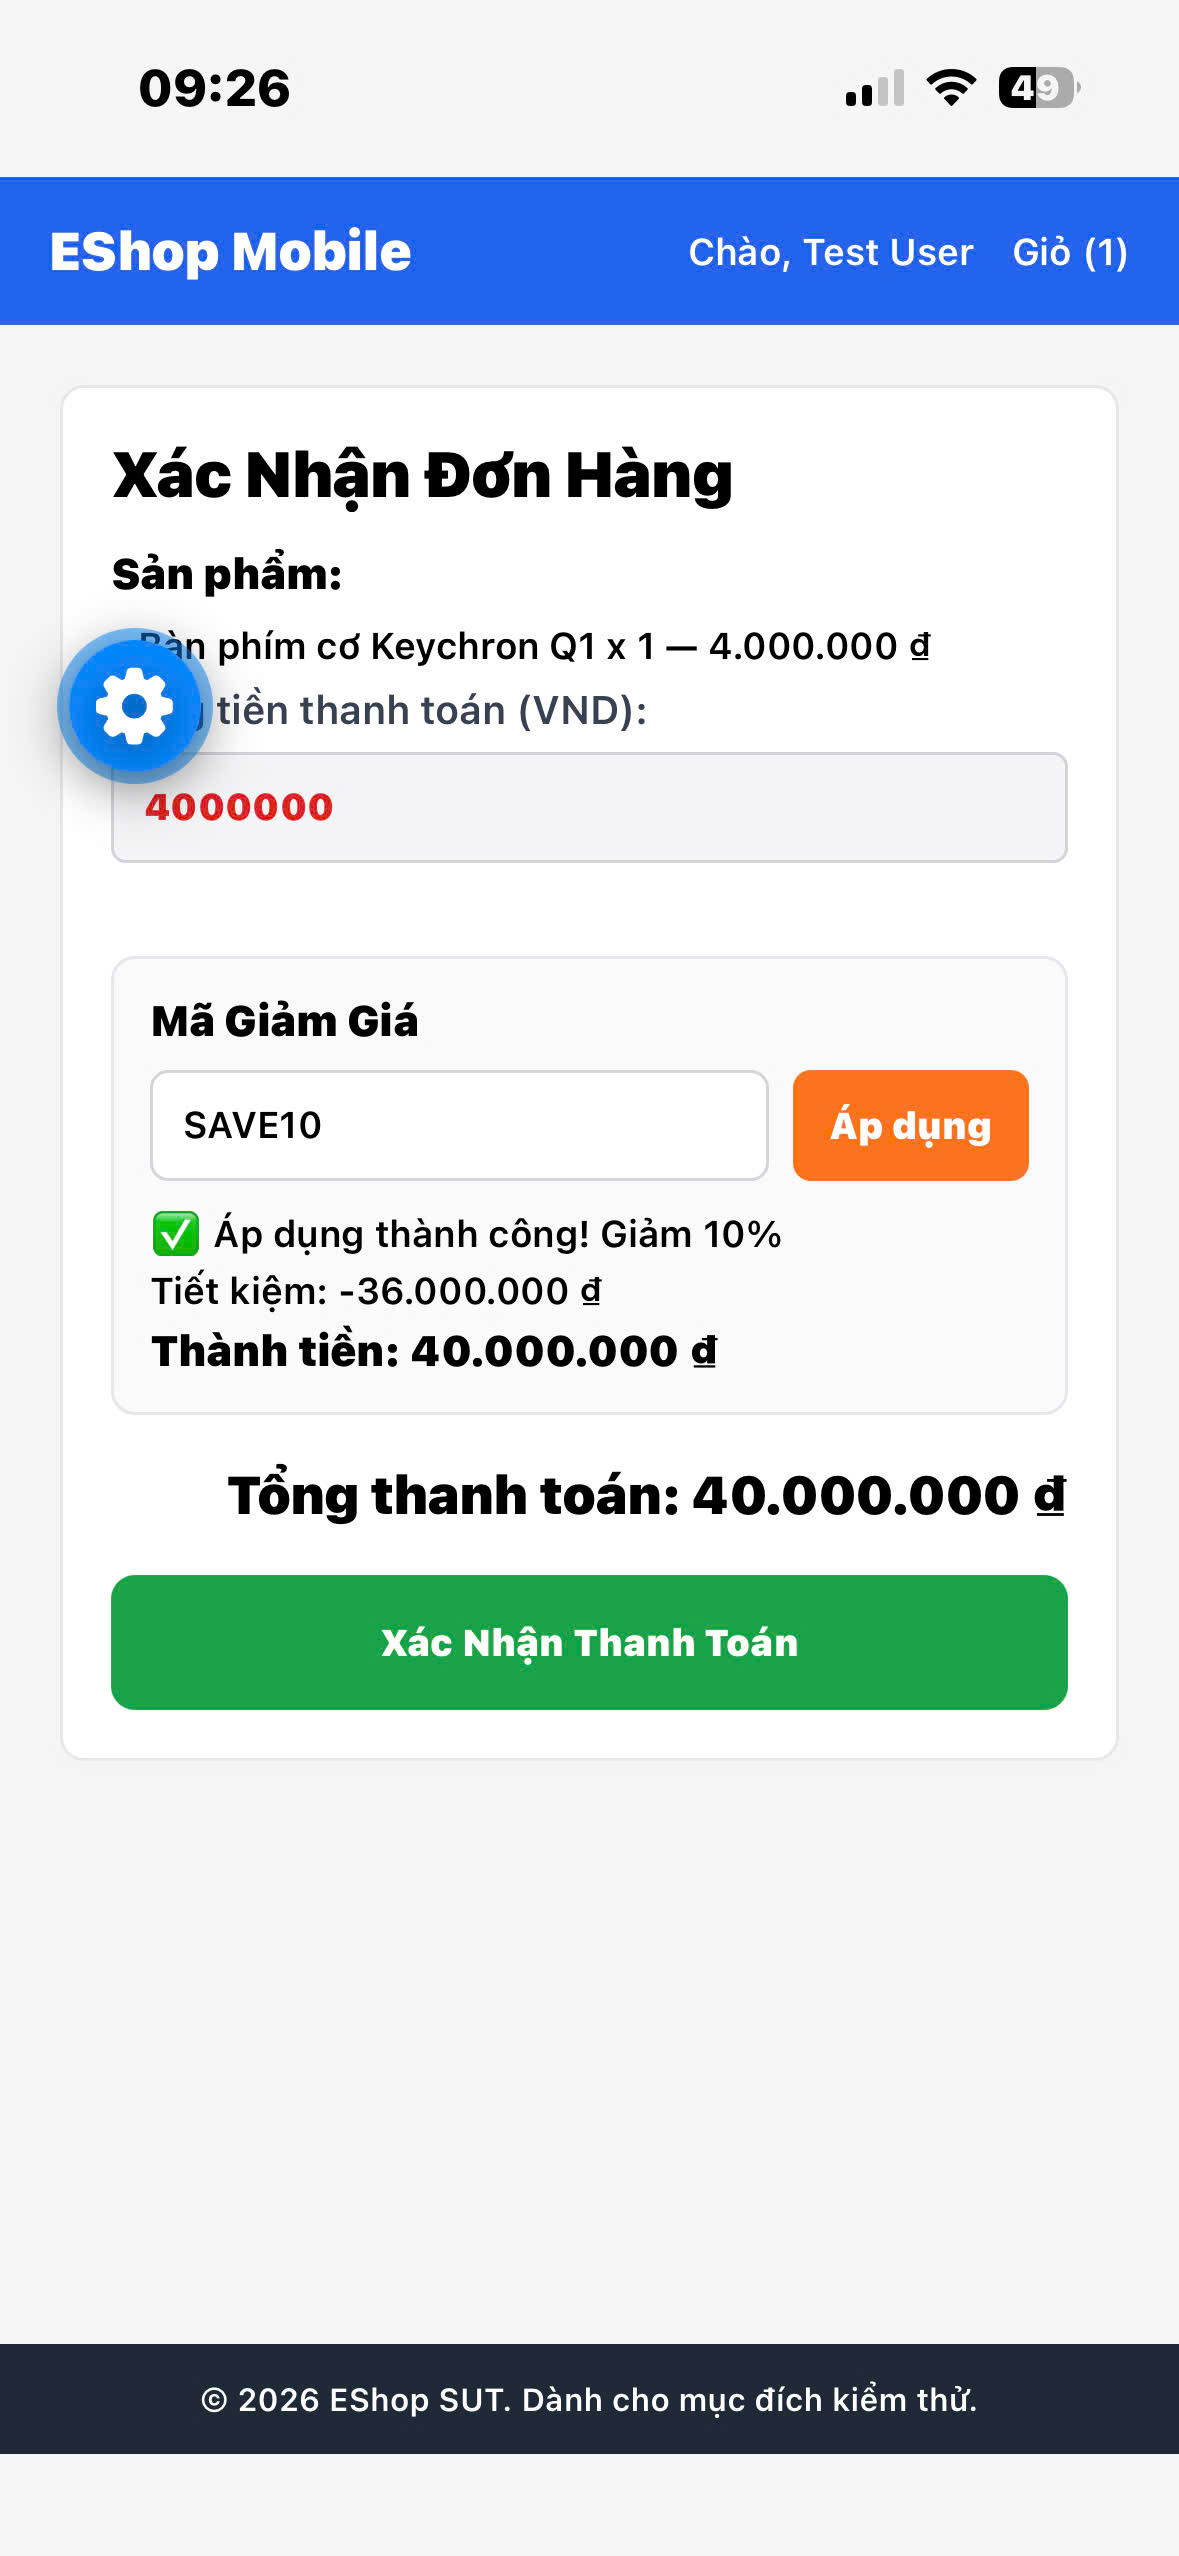
\includegraphics[width=0.42\textwidth,height=0.60\textheight,keepaspectratio]{../../evidence/D/native-ios/screenshots/D-TC-008-ios-physical.jpg}
  \caption{Evidence iOS thật: checkout/keyboard ở D-TC-001 và percent formula sai ở D-TC-008 (modified data).}
  \label{fig:d-native-ios-core}
\end{figure}

\begin{figure}[H]
  \centering
  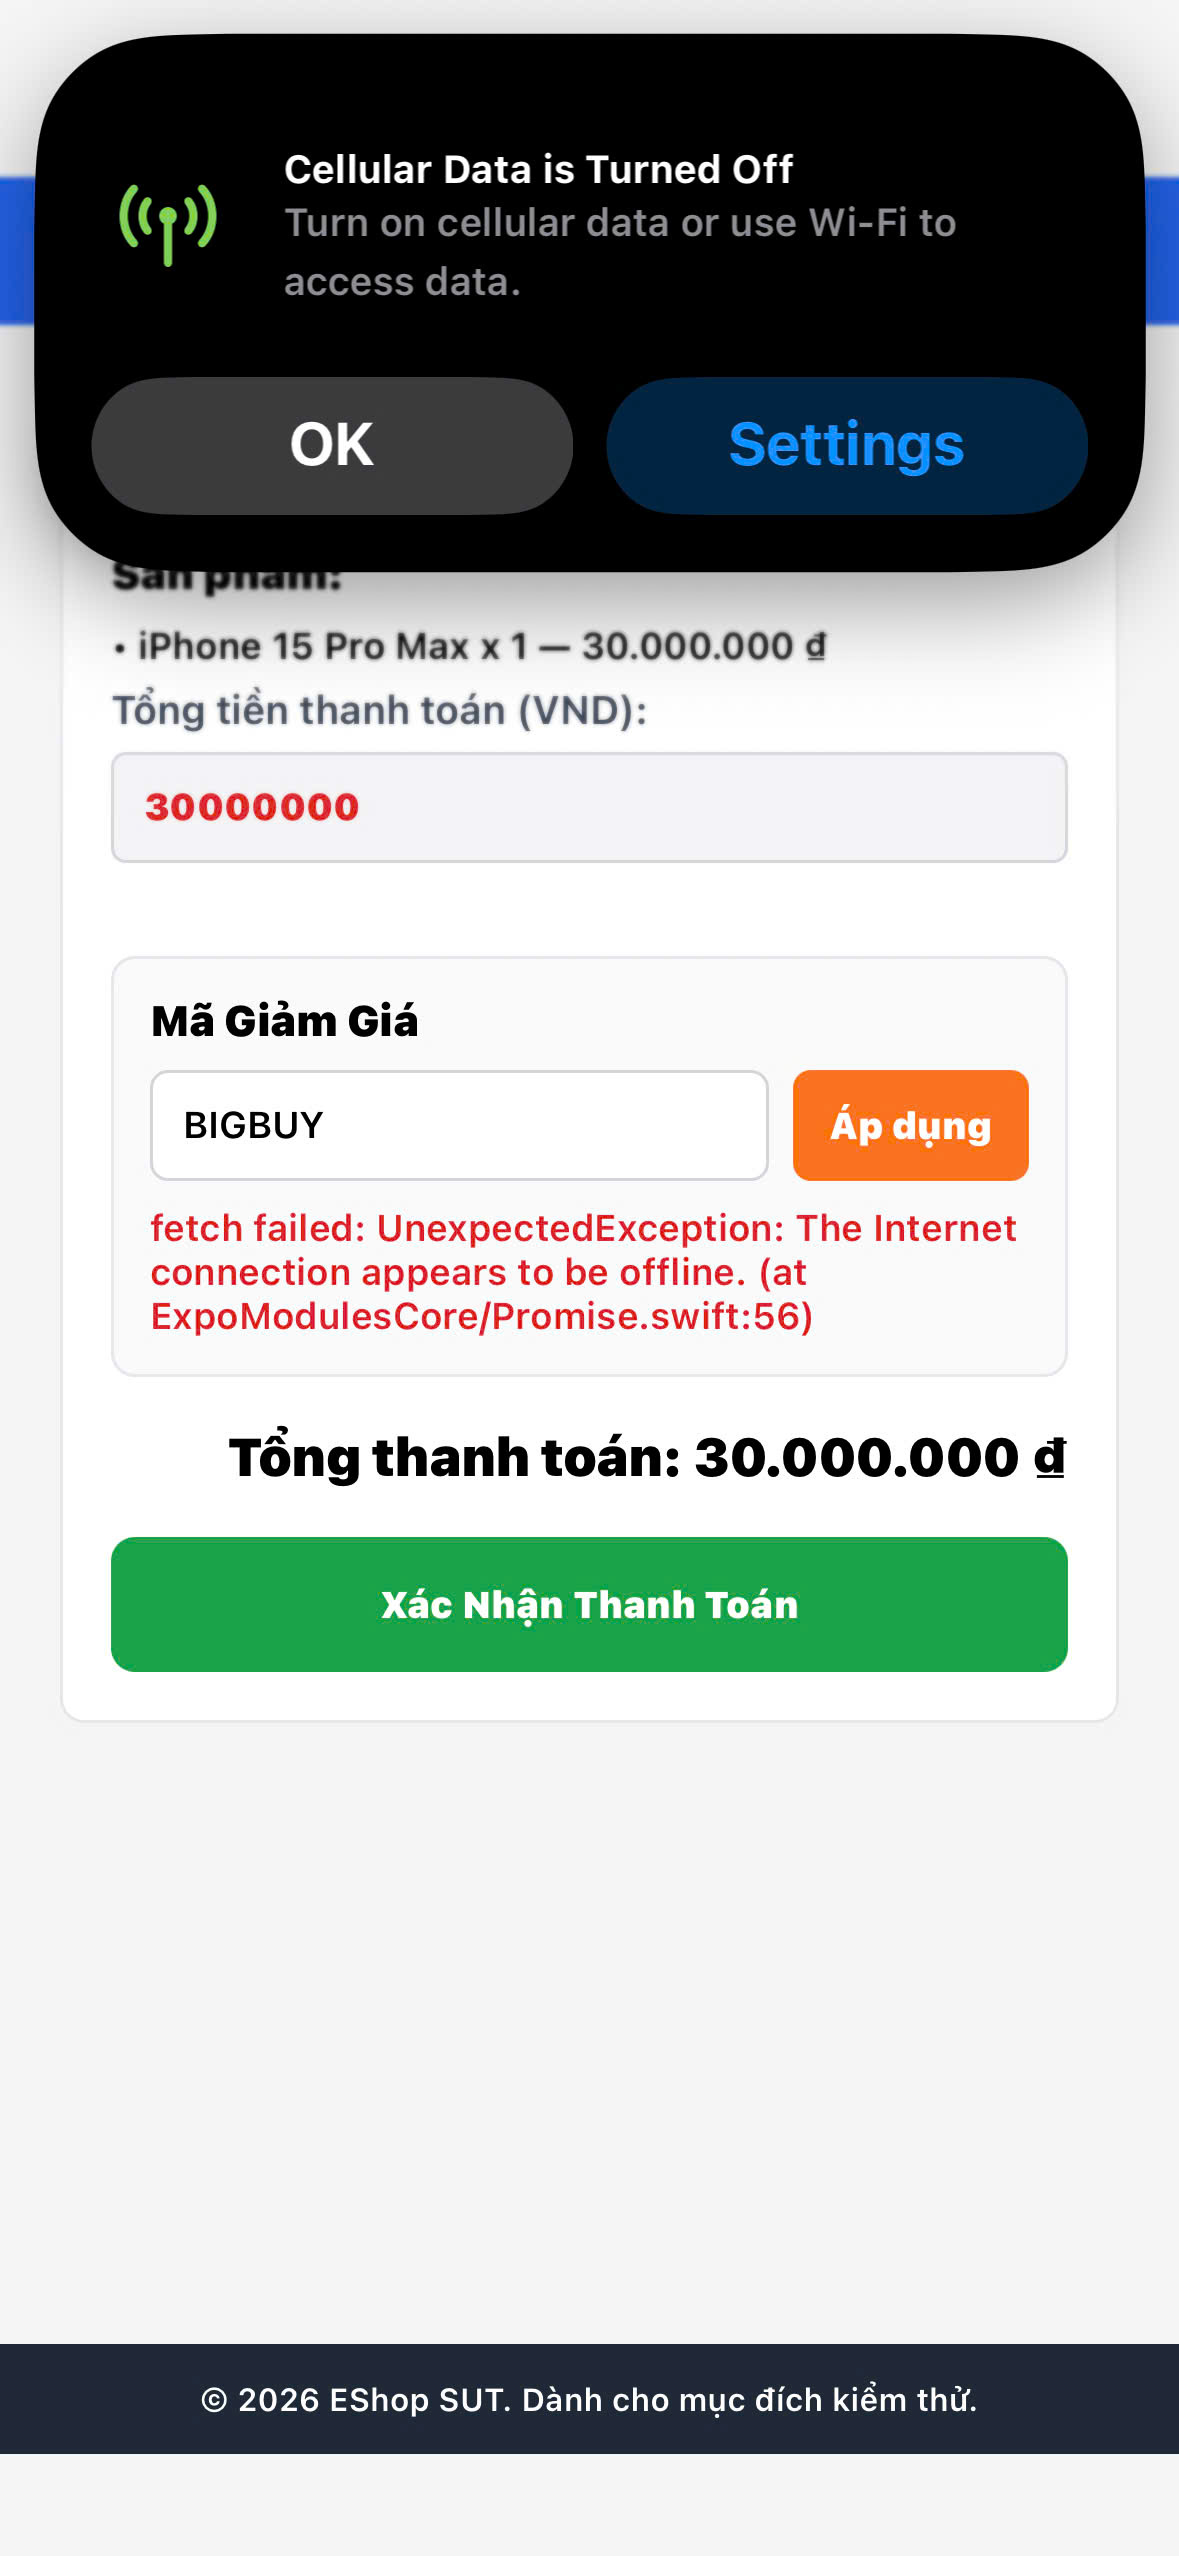
\includegraphics[width=0.42\textwidth,height=0.60\textheight,keepaspectratio]{../../evidence/D/native-ios/screenshots/D-TC-042-ios-physical.jpg}
  \caption{D-TC-042 observation: mất kết nối làm Mobile hiển thị raw transport exception; case vẫn BLOCKED do thiếu network-message oracle.}
  \label{fig:d-native-ios-network}
\end{figure}

\begin{figure}[H]
  \centering
  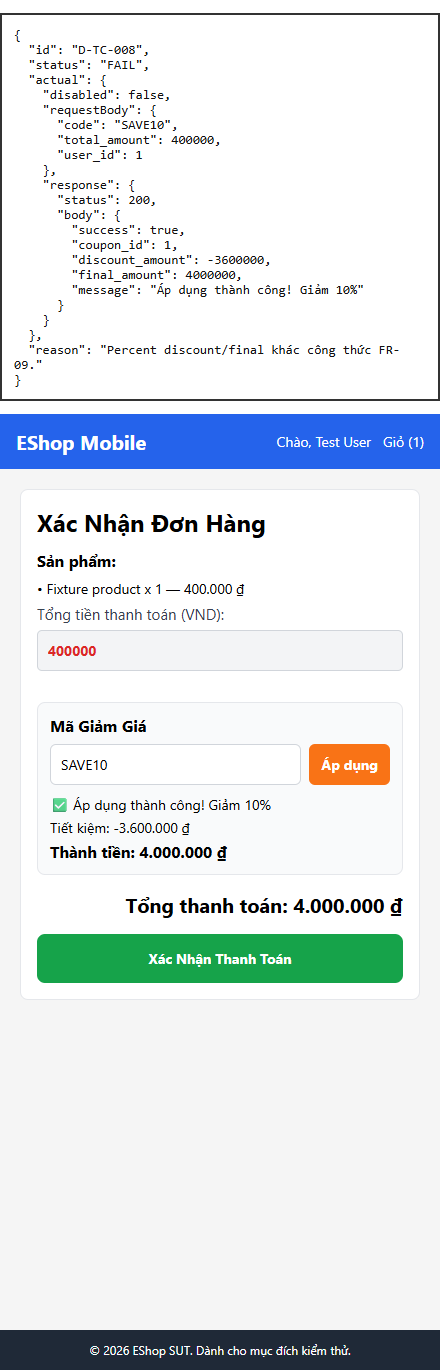
\includegraphics[width=0.76\textwidth,height=0.62\textheight,keepaspectratio]{../../evidence/D/execution/screenshots/D-TC-008.png}
  \caption{D-TC-008 FAIL: công thức percent tạo discount âm và final tăng.}
  \label{fig:d-tc-008-percent-fail}
\end{figure}

\begin{figure}[H]
  \centering
  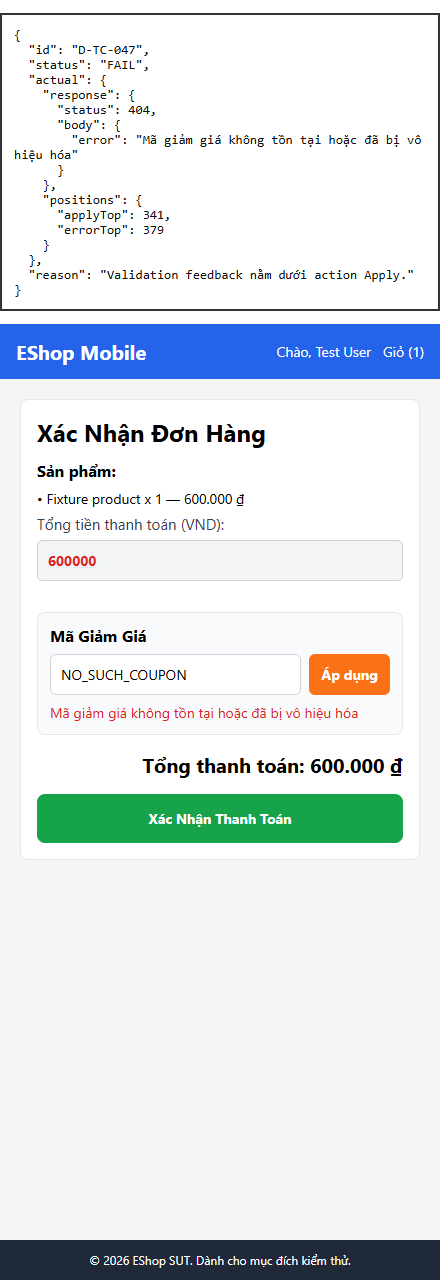
\includegraphics[width=0.76\textwidth,height=0.62\textheight,keepaspectratio]{../../evidence/D/execution/screenshots/D-TC-047.png}
  \caption{D-TC-047 FAIL: validation feedback nằm dưới action Apply.}
  \label{fig:d-tc-047-error-placement}
\end{figure}

\section{Defect và gap}

Mười một FAIL được nhóm thành bảy root cause. Năm lỗi Backend đã có canonical
record \texttt{B-BUG-001}--\texttt{B-BUG-005}; Pool D dẫn lại các ID này với
evidence Mobile thay vì tạo lỗi Backend trùng. Hai lỗi riêng Mobile là
\texttt{D-BUG-001} (sai màu positive action) và \texttt{D-BUG-002} (error nằm
dưới Apply).

\begin{table}[H]
  \centering
  \small
  \begin{tabular}{p{0.18\textwidth}p{0.48\textwidth}p{0.12\textwidth}p{0.10\textwidth}}
    \toprule
    Canonical ID & Root cause ảnh hưởng Pool D & Severity & Case D \\
    \midrule
    B-BUG-001 & Sai công thức percent & Critical & 008, 031 \\
    B-BUG-002 & Sai equality tại minimum & Medium & 017 \\
    B-BUG-003 & Tin total client tại apply/checkout & Critical & 019, 020, 044 \\
    B-BUG-004 & Apply thiếu authentication & High & 027, 028 \\
    B-BUG-005 & Tin body user identity & Critical & 026 \\
    D-BUG-001 & Sai màu positive action Mobile & Low & 046 \\
    D-BUG-002 & Error nằm dưới Apply trên Mobile & Low & 047 \\
    \bottomrule
  \end{tabular}
  \caption{Bảy root-cause group được xác nhận từ 11 FAIL của D-M09.}
  \label{tab:d-m09-defects}
\end{table}

Gap analysis ghi nhận 11 requirement gap, bốn implementation risk, hai
Mobile/environment gap, hai testability gap và sáu blocked condition. Hai mươi
case BLOCKED không được chuyển thành defect.

\section{Traceability, coverage và residual risk}

Ma trận \path{features/D/07_traceability_matrix.md} liên kết từng
\texttt{D-TC-001}--\texttt{D-TC-050} theo chuỗi requirement--partition--boundary--
result--defect/gap--Mobile evidence. Evidence gồm 50 screenshot, 50 trace,
\texttt{results.json}, service log và 9 screenshot iOS thật bổ sung.

Residual risk ở mức rất cao: lỗi công thức tài chính, trusted total,
authentication và identity vẫn tồn tại; minimum equality sai; native behavior
mới được kiểm chứng một phần. Các nhóm chưa có verdict gồm exact expiry, normalization,
rounding/cap/floor, loading/reset state, network resilience và native
viewport/keyboard/accessibility. Kết nối LAN hoạt động trên một thiết bị iOS,
nhưng Android, rotation, accessibility tree và native automation chưa được kiểm chứng.

\section{Kết luận Pool D}

Workflow D-M09 hoàn tất về mặt kỹ thuật với baseline Expo Web và evidence iOS
bổ sung giới hạn: có oracle,
domain model, EP/BVA, 50 test case, automation, evidence, defect/gap analysis,
traceability và nội dung báo cáo. Feature \textbf{không được kết luận hoạt động
đúng} vì còn 11 FAIL, 20 BLOCKED và chưa có coverage native có kiểm soát trên
iOS/Android. Cần sửa defect, chốt gap và regression trước khi chấp nhận chất lượng.
